% The punctured plane U (right) with O_U(U)=k[x,y] and its two axis-divisors
% V(x), V(y); beside a hypothetical Spec B (left) with crossing divisors
% V(a), V(b) meeting at a point (a,b).
% Source: book/tex/alg-geom/mor-scheme.tex (Prop: punctured plane isn't affine).
\documentclass[border=2mm]{standalone}
\usepackage{tikz,amssymb,amsmath}
\begin{document}
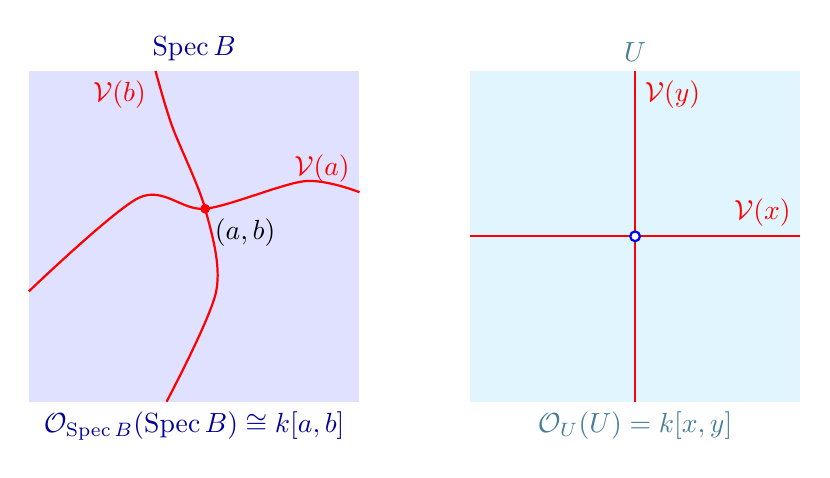
\begin{tikzpicture}[scale=0.7]
  % ---- left panel: Spec B ----
  \begin{scope}[xshift=-8cm]
    \fill[blue!12] (-3,-3) rectangle (3,3);
    \draw[red, thick] plot[smooth] coordinates {(-3,-1) (-1,0.7) (0.2,0.5) (2,1) (3,0.8)};
    \draw[red, thick] plot[smooth] coordinates {(-0.5,-3) (0.4,-1) (0.2,0.5) (-0.4,2) (-0.7,3)};
    \fill[red] (0.2,0.5) circle (2.5pt) node[below right, black]{$(a,b)$};
    \node[red] at (3,0.8) [above left]{$\mathcal V(a)$};
    \node[red] at (-0.7,3) [below left]{$\mathcal V(b)$};
    \node[blue!60!black] at (0,3) [above]{$\operatorname{Spec} B$};
    \node[blue!60!black] at (0,-3) [below]{$\mathcal O_{\operatorname{Spec} B}(\operatorname{Spec} B)\cong k[a,b]$};
  \end{scope}
  % ---- right panel: U (punctured plane) ----
  \fill[cyan!12] (-3,-3) rectangle (3,3);
  \draw[red, thick] (0,-3)--(0,3);
  \draw[red, thick] (-3,0)--(3,0);
  \draw[blue, thick, fill=white] (0,0) circle (2.5pt);
  \node[red] at (3,0) [above left]{$\mathcal V(x)$};
  \node[red] at (0,3) [below right]{$\mathcal V(y)$};
  \node[cyan!55!black] at (0,3) [above]{$U$};
  \node[cyan!55!black] at (0,-3) [below]{$\mathcal O_U(U)=k[x,y]$};
\end{tikzpicture}
\end{document}
